\begin{figure} [!h]
	
  \setlength{\unitlength}{\textwidth}

        \begin{picture}(0.9,0.8)(0.06,0.3)

      % % % Parkinson Data 

      \put(0.05,0.39){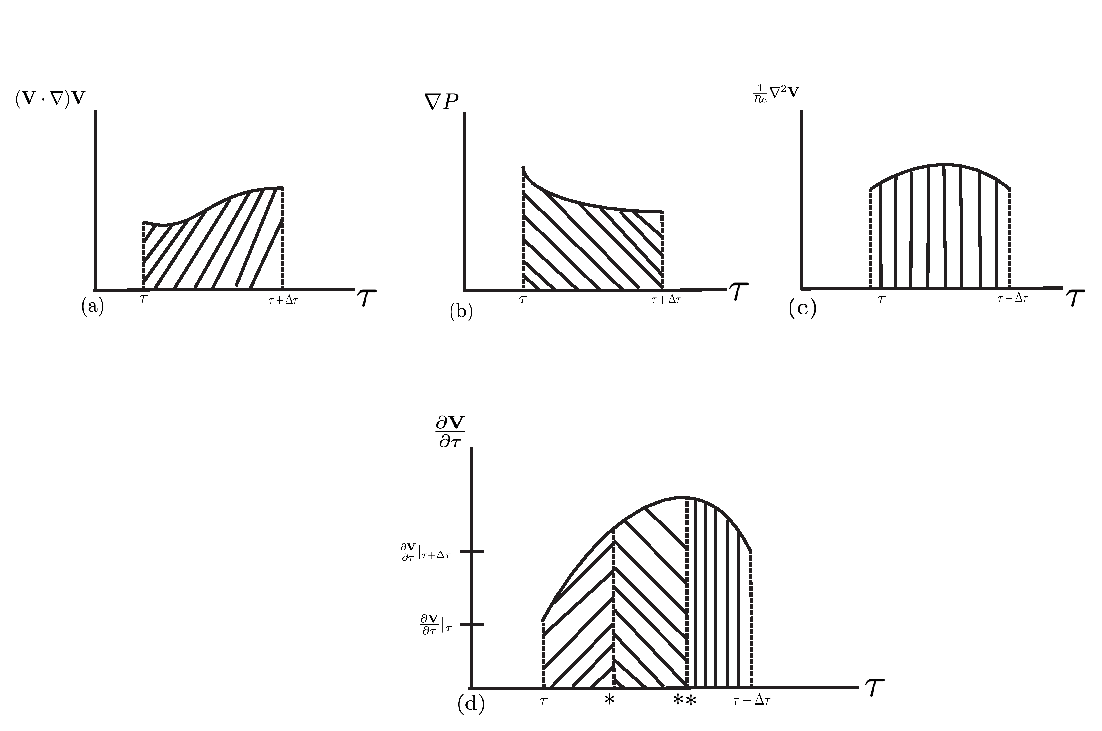
\includegraphics[width=0.93\unitlength]{./chapter-methodology/fnp/convection.eps}}
      
%       \put(0.07,0.95){$\displaystyle\frac{V}{D}$}
%       \put(0.07,1.3){$\displaystyle\frac{A}{D}$}
  
       \
%\put(0.189,1.415){\small(a)}
%\put(0.189,1.07){\small(b)}
%\put(0.189,0.73){\small(c)}

%  


    \end{picture}

  \caption{Sketch of the integration of the time splitting scheme.(a), (b) and (c) represents the convection pressure and diffusion sub steps. The intermediate time steps are represented by (\ding{83}) and (\ding{83} \ding{83}) }
    \label{fig:convection-sketch}
\end{figure}

 %vspace{10cm}
